\documentclass[journal,12pt,twocolumn]{IEEEtran}
%
\usepackage{setspace}
\usepackage{gensymb}
\usepackage{siunitx}
\usepackage{tkz-euclide} 
\usepackage{textcomp}
\usepackage{standalone}
\usetikzlibrary{calc}
\newcommand\hmmax{0}
\newcommand\bmmax{0}

%\doublespacing
\singlespacing

%\usepackage{graphicx}
%\usepackage{amssymb}
%\usepackage{relsize}
\usepackage[cmex10]{amsmath}
%\usepackage{amsthm}
%\interdisplaylinepenalty=2500
%\savesymbol{iint}
%\usepackage{txfonts}
%\restoresymbol{TXF}{iint}
%\usepackage{wasysym}
\usepackage{amsthm}
%\usepackage{iithtlc}
\usepackage{mathrsfs}
\usepackage{txfonts}
\usepackage{stfloats}
\usepackage{bm}
\usepackage{cite}
\usepackage{cases}
\usepackage{subfig}
%\usepackage{xtab}
\usepackage{longtable}
\usepackage{multirow}
%\usepackage{algorithm}
%\usepackage{algpseudocode}
\usepackage{enumitem}
\usepackage{mathtools}
\usepackage{steinmetz}
\usepackage{tikz}
\usepackage{circuitikz}
\usepackage{verbatim}
\usepackage{tfrupee}
\usepackage[breaklinks=true]{hyperref}
%\usepackage{stmaryrd}
\usepackage{tkz-euclide} % loads  TikZ and tkz-base
%\usetkzobj{all}
\usetikzlibrary{calc,math}
\usepackage{listings}
    \usepackage{color}                                            %%
    \usepackage{array}                                            %%
    \usepackage{longtable}                                        %%
    \usepackage{calc}                                             %%
    \usepackage{multirow}                                         %%
    \usepackage{hhline}                                           %%
    \usepackage{ifthen}                                           %%
  %optionally (for landscape tables embedded in another document): %%
    \usepackage{lscape}     
\usepackage{multicol}
\usepackage{chngcntr}
\usepackage{amsmath}
\usepackage{cleveref}
\usepackage{amsmath}
%\usepackage{enumerate}

%\usepackage{wasysym}
%\newcounter{MYtempeqncnt}
\DeclareMathOperator*{\Res}{Res}
%\renewcommand{\baselinestretch}{2}
\renewcommand\thesection{\arabic{section}}
\renewcommand\thesubsection{\thesection.\arabic{subsection}}
\renewcommand\thesubsubsection{\thesubsection.\arabic{subsubsection}}

\renewcommand\thesectiondis{\arabic{section}}
\renewcommand\thesubsectiondis{\thesectiondis.\arabic{subsection}}
\renewcommand\thesubsubsectiondis{\thesubsectiondis.\arabic{subsubsection}}

% correct bad hyphenation here
\hyphenation{op-tical net-works semi-conduc-tor}
\def\inputGnumericTable{}                                 %%

\lstset{
%language=C,
frame=single, 
breaklines=true,
columns=fullflexible
}
%\lstset{
%language=tex,
%frame=single, 
%breaklines=true
%}
\usepackage{graphicx}
\usepackage{pgfplots}

\begin{document}


\newtheorem{theorem}{Theorem}[section]
\newtheorem{problem}{Problem}
\newtheorem{proposition}{Proposition}[section]
\newtheorem{lemma}{Lemma}[section]
\newtheorem{corollary}[theorem]{Corollary}
\newtheorem{example}{Example}[section]
\newtheorem{definition}[problem]{Definition}
%\newtheorem{thm}{Theorem}[section] 
%\newtheorem{defn}[thm]{Definition}
%\newtheorem{algorithm}{Algorithm}[section]
%\newtheorem{cor}{Corollary}
\newcommand{\BEQA}{\begin{eqnarray}}
\newcommand{\EEQA}{\end{eqnarray}}
\newcommand{\define}{\stackrel{\triangle}{=}}
\bibliographystyle{IEEEtran}
%\bibliographystyle{ieeetr}
\providecommand{\mbf}{\mathbf}
\providecommand{\abs}[1]{\ensuremath{\left\vert#1\right\vert}}
\providecommand{\norm}[1]{\ensuremath{\left\lVert#1\right\rVert}}
\providecommand{\mean}[1]{\ensuremath{E\left[ #1 \right]}}
\providecommand{\pr}[1]{\ensuremath{\Pr\left(#1\right)}}
\providecommand{\qfunc}[1]{\ensuremath{Q\left(#1\right)}}
\providecommand{\sbrak}[1]{\ensuremath{{}\left[#1\right]}}
\providecommand{\lsbrak}[1]{\ensuremath{{}\left[#1\right.}}
\providecommand{\rsbrak}[1]{\ensuremath{{}\left.#1\right]}}
\providecommand{\brak}[1]{\ensuremath{\left(#1\right)}}
\providecommand{\lbrak}[1]{\ensuremath{\left(#1\right.}}
\providecommand{\rbrak}[1]{\ensuremath{\left.#1\right)}}
\providecommand{\cbrak}[1]{\ensuremath{\left\{#1\right\}}}
\providecommand{\lcbrak}[1]{\ensuremath{\left\{#1\right.}}
\providecommand{\rcbrak}[1]{\ensuremath{\left.#1\right\}}}
\theoremstyle{remark}
\newtheorem{rem}{Remark}
\newcommand{\sgn}{\mathop{\mathrm{sgn}}}
\providecommand{\res}[1]{\Res\displaylimits_{#1}} 
%\providecommand{\norm}[1]{\lVert#1\rVert}
\providecommand{\mtx}[1]{\mathbf{#1}}
\providecommand{\fourier}{\overset{\mathcal{F}}{ \rightleftharpoons}}
%\providecommand{\hilbert}{\overset{\mathcal{H}}{ \rightleftharpoons}}
\providecommand{\system}{\overset{\mathcal{H}}{ \longleftrightarrow}}
	%\newcommand{\solution}[2]{\textbf{Solution:}{#1}}
\newcommand{\solution}{\noindent \textbf{Solution: }}
\newcommand{\cosec}{\,\text{cosec}\,}
\providecommand{\dec}[2]{\ensuremath{\overset{#1}{\underset{#2}{\gtrless}}}}
\newcommand{\myvec}[1]{\ensuremath{\begin{pmatrix}#1\end{pmatrix}}}
\newcommand{\mydet}[1]{\ensuremath{\begin{vmatrix}#1\end{vmatrix}}}
%\numberwithin{equation}{section}
\numberwithin{equation}{subsection}
%\numberwithin{problem}{section}
%\numberwithin{definition}{section}
\makeatletter
\@addtoreset{figure}{problem}
\makeatother
\let\StandardTheFigure\thefigure
\let\vec\mathbf
%\renewcommand{\thefigure}{\theproblem.\arabic{figure}}
\renewcommand{\thefigure}{\theproblem}
%\setlist[enumerate,1]{before=\renewcommand\theequation{\theenumi.\arabic{equation}}
%\counterwithin{equation}{enumi}
%\renewcommand{\theequation}{\arabic{subsection}.\arabic{equation}}
\def\putbox#1#2#3{\makebox[0in][l]{\makebox[#1][l]{}\raisebox{\baselineskip}[0in][0in]{\raisebox{#2}[0in][0in]{#3}}}}
     \def\rightbox#1{\makebox[0in][r]{#1}}
     \def\centbox#1{\makebox[0in]{#1}}
     \def\topbox#1{\raisebox{-\baselineskip}[0in][0in]{#1}}
\vspace{3cm}
\title{Polynomial Curve Fitting}
\maketitle
\newpage
%\tableofcontents
\bigskip
\renewcommand{\thefigure}{\theenumi}
\renewcommand{\thetable}{\theenumi}
\begin{abstract}
This document contains theory behind curve fitting model
\end{abstract}
\section{\textbf{Objective}}
Our objective is to implement the best fit line  polynomial Curve.
\section{Load Dataset}
Create a sinusoidal data function
\begin{align}
    y = A\sin{2\pi{ft}}+n\brak{t}
\end{align}
with random noise included in the target values training set comprising N observations of t,
written
\begin{align}
    t=\myvec{t_1 &,&.&.& t_N}^T 
\end{align}
together with corresponding observations of the values
of y, denoted 
\begin{align}
    y=\myvec{y_1 &,&.&.& y_N}^T
\end{align}
\begin{figure}[!h]
\begin{center}
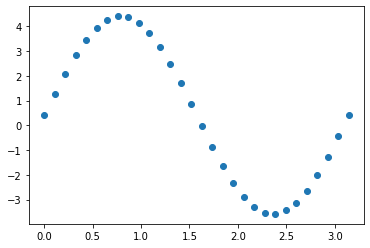
\includegraphics[width=3.4in]{a1.png}
\end{center}
\caption{Sinusoidal Dataset}
\label{fig:1}
\end{figure}
Fig \ref{fig:1} was generated by choosing
values of $t_n$, for n = 1, . . . , N, where N= 30 and spaced uniformly. Data set y was obtained by first computing the corresponding values of the function $A\sin2\pi{ft}$ and then adding a small level of random noise having a Uniform distribution to each such point in order to obtain the corresponding value.
\begin{lstlisting}
# Data Creation
poly_order = 4
# Number of training samples
N = 30
t = np.linspace(0, np.pi, N)
f=1
A=4
# Generate some numbers from the sine function
y = A*np.sin(2*f*t)
# Add noise
y += np.random.RandomState(1).uniform()
#defining it as a matrix
y_1 = np.asmatrix(y.reshape(N,1))
plt.plot(t, y, 'o');
plt.show()
\end{lstlisting}
Adding the bias and higher order terms,
Here column-1 will always be the value of coefficient, which will always be 1. But to create a matrix we need to consider it as a column.
\begin{lstlisting}
B = np.append(np.ones((N,1)),t.reshape((N,1)),axis = 1)
for i in range(0,poly_order-1):
	B = np.append(B,(t.reshape((N,1)))**(i+2),axis = 1)
B = np.asmatrix(B)
print(B.shape)
print(B)
\end{lstlisting}
The matrix we got from the above code,
\begin{align}
\vec{B}= \myvec{ 1 & t_{0} & t_{0}^2 & \ldots & t_{0}^{N-1} \\
		1 & t_{1} & t_{1}^2 & \ldots & t_{1}^{N-1} \\
		1 & t_{2} & t_{2}^2 & \ldots & t_{2}^{N-1} \\
		\vdots & & \vdots &  & \vdots  \\
		    1 & \ldots & \ldots & \ldots & t_{N}^{N-1} }\label{eq:1}
\end{align}
%
\section{Polynomial Curve Fitting}
To find a line that best resembles the underlying pattern of the training data shown in the graph. By using the least squares method to Parameterize our model with the coefficients that best describe the training set before seeing how well the model generalizes to data it hasn’t seen before.
In particular, we shall fit the data using a
polynomial function of the form, where N is the order of the polynomial. 
\begin{align}
y = \sum_{j=0}^{N} w_jt^{j}\\
y = \hat{\vec{w}}\vec{B}\\
y= \hat{\vec{w}}\myvec{ 1 & t_{0} & t_{0}^2 & \ldots & t_{0}^{N-1} \\
		1 & t_{1} & t_{1}^2 & \ldots & t_{1}^{N-1} \\
		1 & t_{2} & t_{2}^2 & \ldots & t_{2}^{N-1} \\
		\vdots & & \vdots &  & \vdots  \\
		    1 & \ldots & \ldots & \ldots & t_{N}^{N-1} }\label{eq:2}
\end{align}
Finding the optimum weights of Model using the \textbf{Normal Equation} an analytical approach to Polynomial Regression with a Least Square Cost Function, using \eqref{eq:1}
\begin{align}
    \hat{\vec{w}} = \brak{\vec{B}^T\vec{B}}^{-1}\brak{\vec{B}^Ty}
\end{align}
where,
\\
$\hat{\vec{w}}$: is hypothesis parameters that define it the best.
\\
$\vec{B}$: Input feature value of each instance
\\
y: Output value of each instance.
\begin{lstlisting}
w = (B.T*B).I*B.T*y_1
print(w)
\end{lstlisting} 
%Form the above the weight matrix we get,
%\begin{align}
%    \vec{w} = \myvec{w_{0} & w_{1} & w_{2} &  w_{3} & \ldots %& w_{N}}^T \label{eq:3}
%\end{align}
%Substituting \eqref{eq:1} and \eqref{eq:3} in Eq. \eqref{eq:2}
%we get, 
%\begin{align}
%    y= \myvec{w_{0} \\ w_{1} \\ w_{2}  \\ \ldots \\ w_{N}} \myvec{ 1 & t_{0} & t_{0}^2 & \ldots & t_{0}^{N-1} \\
%		1 & t_{1} & t_{1}^2 & \ldots & t_{1}^{N-1} \\
%		1 & t_{2} & t_{2}^2 & \ldots & t_{2}^{N-1} \\
%		\vdots & & \vdots &  & \vdots  \\
%		    1 & \ldots & \ldots & \ldots & t_{N}^{N-1} %}\label{eq:4}
%\end{align}
%
Multiplying the above matrix  named is as y-pred,
\begin{lstlisting}
y_pred = B * w
y_pred
print(y_pred.shape)
\end{lstlisting}
Now we quantify how well our model fits the data by using the least squared error (LSE) to calculate the average squared difference between our line and the actual data point in the training set.
\begin{lstlisting}
def LSE_error(y_pred,y_1):
  var = (y_1-y_pred)
  n = len(var)
  MSE= np.asmatrix(y_1-y_pred).T*np.asmatrix(y_1-y_pred)
  MSE = (MSE/n)
  return MSE
  
  error1 = LSE_error(y_1,y_pred)
print(error1)
\end{lstlisting}
\begin{figure}[!h]
\begin{center}
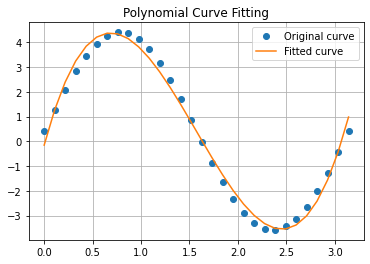
\includegraphics[width=3.4in]{a2.png}
\end{center}
\caption{Fitted Data}
\label{fig:2}
\end{figure}
To plot the Predicted and actual plot 
\begin{lstlisting}
plt.plot(t,y_1,'o',label = 'Original curve')
plt.plot(t,y_pred,label = 'Fitted curve')
plt.legend()
plt.grid()
plt.title("Polynomial Curve Fitting")
plt.show()
\end{lstlisting}
\section{Observation}
\begin{itemize}
  \item Model is approximated by a polynomial function
  \item Noise is added to the training data labels
  \item With polynomial degree N= 1, we got LSE of 3.51.
  \item with polynomial degree N= 4 we got LSE of 0.0888215
  \item with polynomial degree N= 10 we got LSE of 1.29225829e-07
\end{itemize}
Clearly as the number of parameters crosses the number of training points, the model is performing very poorly
\end{document}
